\documentclass{article}
\usepackage{pgfplots}
\pgfplotsset{compat=1.18}

\begin{document}

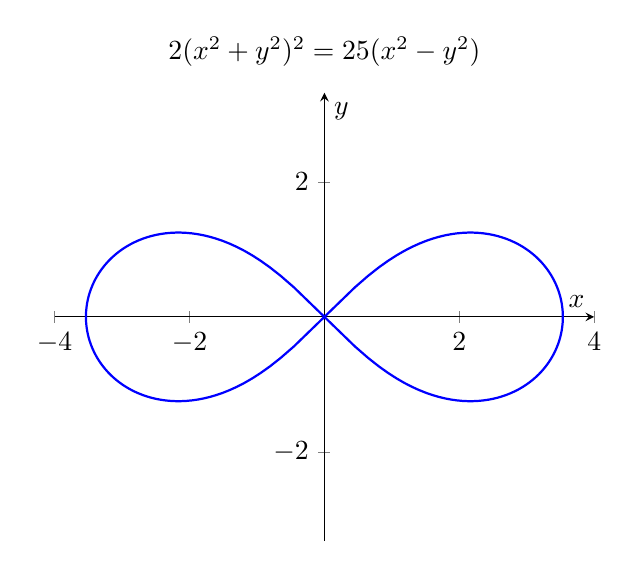
\begin{tikzpicture}
\begin{axis}[
    title={$2(x^2+y^2)^2 = 25(x^2-y^2)$},
    axis lines=center, % Puts the axes in the middle
    xlabel={$x$},
    ylabel={$y$},
    xmin=-4, xmax=4,
    ymin=-2, ymax=2,
    axis equal, % Crucial: Ensures the figure-8 isn't stretched or squished
    samples=100, % Higher number = smoother curve
    domain=-45:45 % Domain for the right lobe
]

% Right Lobe
\addplot [
    thick, 
    color=blue
] 
({sqrt(12.5*cos(2*x)) * cos(x)}, {sqrt(12.5*cos(2*x)) * sin(x)});

% Left Lobe
\addplot [
    thick, 
    color=blue,
    domain=135:225 % Domain for the left lobe
] 
({sqrt(12.5*cos(2*x)) * cos(x)}, {sqrt(12.5*cos(2*x)) * sin(x)});

\end{axis}
\end{tikzpicture}

\end{document}